% ============================================================
%  N.2.4  Eyeriss CS1 — WReg Sensitivity and Feasibility
% ============================================================
\subsection{Eyeriss: Weight Register Sensitivity (CS1)}
\label{sec:ey-cs1}

\subsubsection{Motivation}

In the Eyeriss-Like architecture every PE stores its assigned weight
filters in a local Weight Register (WReg).
When multiple layers are fused, a single PE must hold the weight
residuals for \emph{all} fused layers simultaneously, that is, the
$C_i \times R_i$ factor products that are not spatially absorbed by
the SARows mapping.
The WReg is therefore the largest per-PE register, ranging from
roughly 460 to over 14\,000 entries depending on the PE configuration,
and it acts as the binding constraint on feasibility: if the required
weight footprint exceeds the WReg capacity, no valid mapping exists
for that PE configuration.

There is a direct trade-off between WReg size and the minimum number
of PEs:
%
\begin{itemize}
  \item A \emph{smaller} WReg forces the mapper to use more PE rows so
        that more weight factors are spatially absorbed, increasing the
        total PE count (and thus area).
  \item A \emph{larger} WReg allows each PE to store more residual
        weight data, reducing the minimum required PE rows and total PE
        count, at the cost of higher per-PE register energy.
\end{itemize}
%
CS1 sweeps three WReg sizes per workload and, for each size,
exhaustively searches over all PE configurations (rows and columns up
to a total of 17\,000~PEs) to determine which configurations are
feasible.
Two summaries are extracted:
%
\begin{description}
  \item[Summary~A (minimum PEs):] the feasible configuration with the
    fewest total PEs, irrespective of EDP.
  \item[Summary~B (minimum EDP):] the feasible configuration with the
    lowest EDP, which may require more PEs than Summary~A.
\end{description}
%
All other registers (InReg, IntReg, OutReg) and the GlobalBuffer
(128\,KB) are held constant at their canonical per-workload values,
and the tile size is fixed at~1.

\subsubsection{Results}

\paragraph{Feasibility and minimum PEs.}
Figure~\ref{fig:ey-cs1-feas} shows, for each workload, the number of
feasible PE configurations (bars) and the minimum total PE count (red
diamonds) as a function of WReg size.

\begin{figure}[htbp]
  \centering
  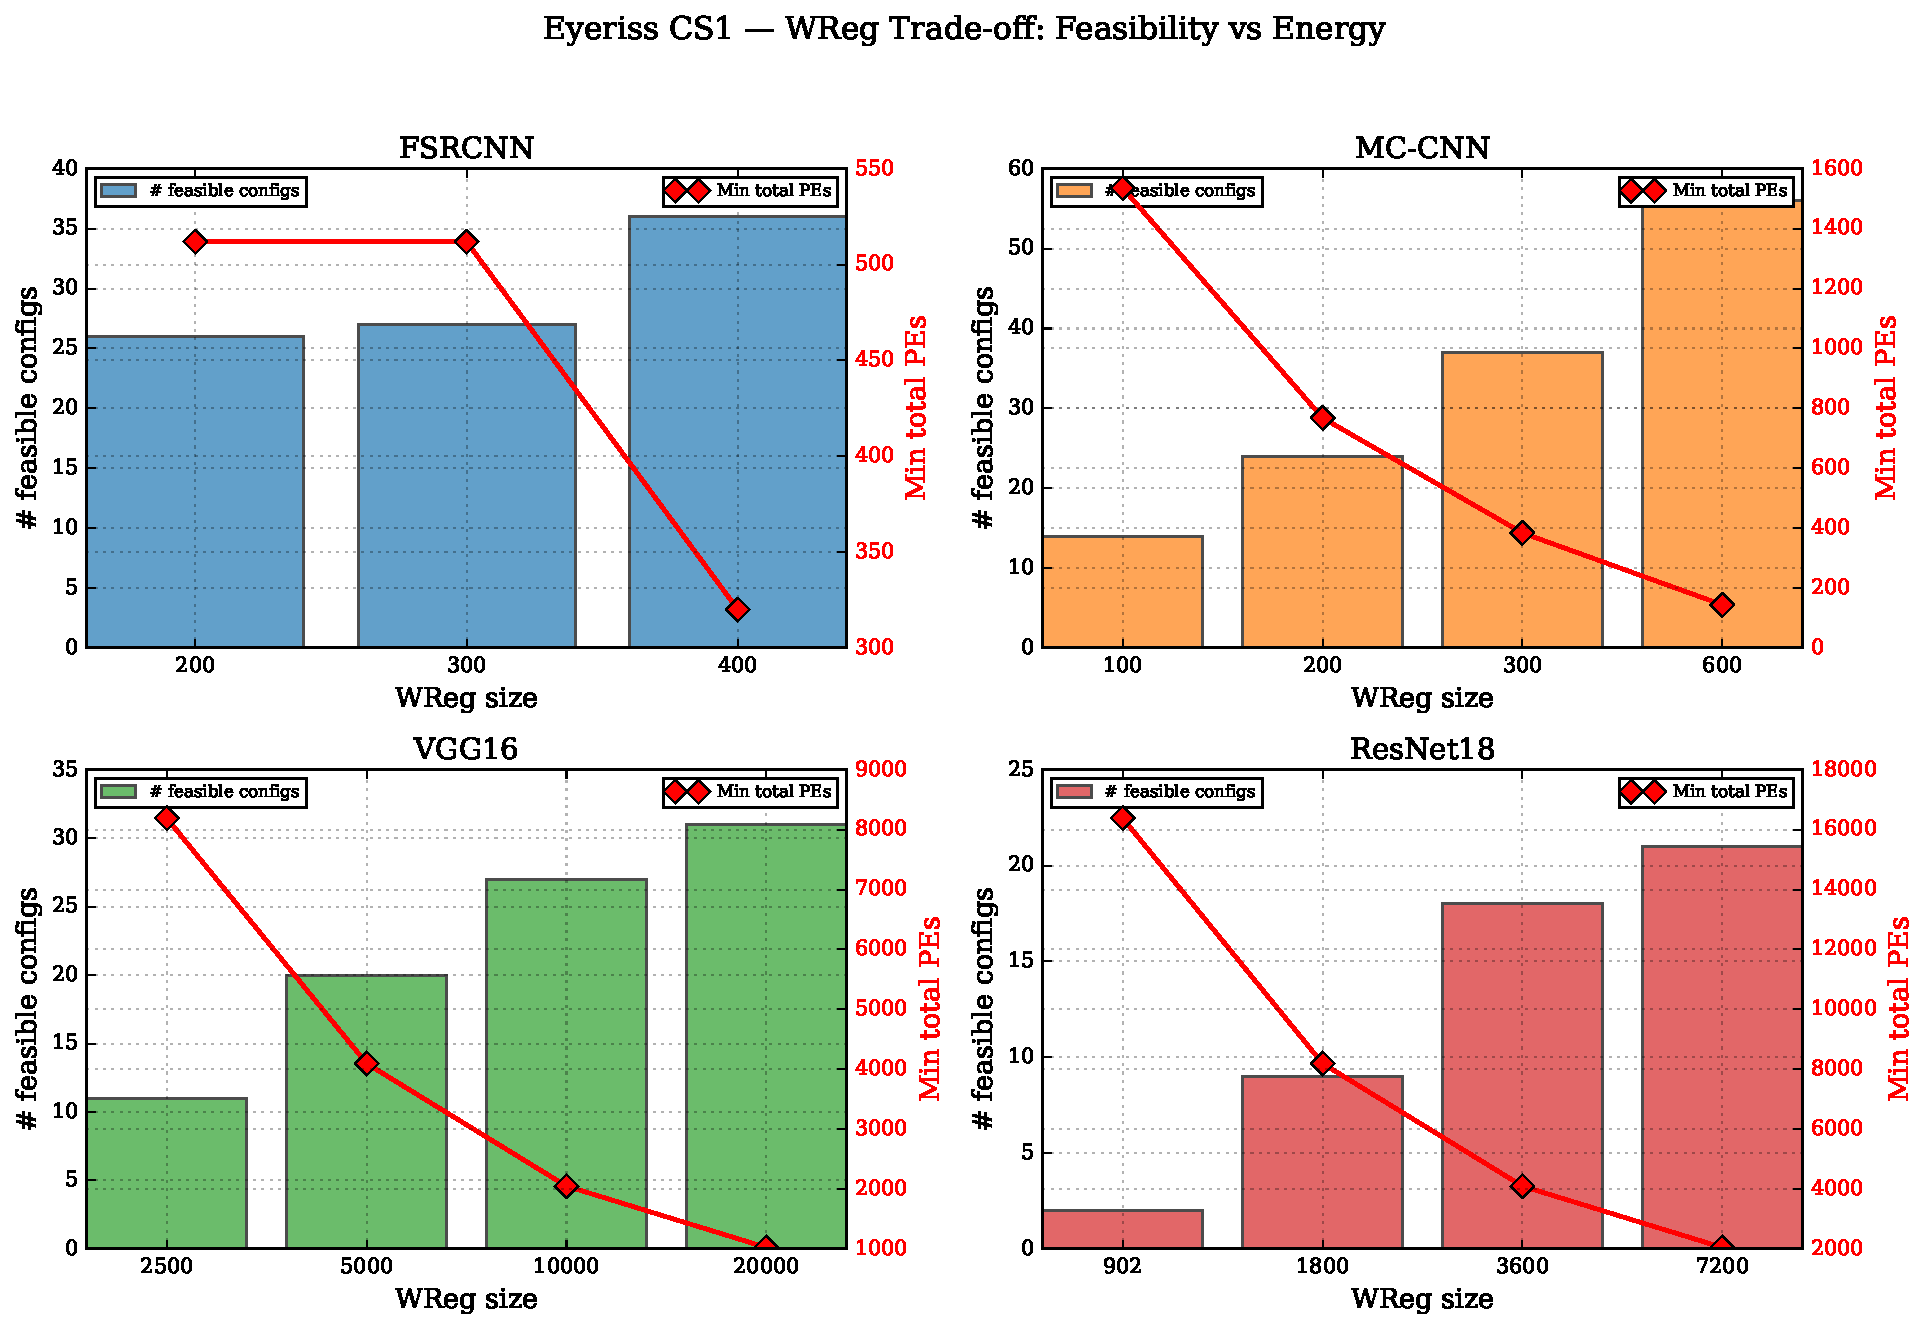
\includegraphics[width=0.85\textwidth]{plots/eyeriss_cs1_wreg_feasibility.pdf}
  \caption{Eyeriss CS1 — WReg trade-off: number of feasible PE
    configurations and minimum PE count vs.\ WReg size.}
  \label{fig:ey-cs1-feas}
\end{figure}

Taking ResNet18 as an example, at WReg\,=\,902 (the smallest tested
value) only 2~out of the full PE grid are feasible, both requiring
16\,384~PEs ($256 \times 64$).
Doubling the WReg to 1\,800 increases the feasible set to 6
configurations and halves the minimum PE count to 8\,192
($128 \times 64$).
A further doubling to 3\,600 yields 8~feasible configurations and
reduces the minimum to 4\,096 PEs ($128 \times 32$).
The pattern is consistent across workloads: each approximate doubling
of WReg halves the minimum PE count, confirming the inverse
relationship $\text{WReg} \times \text{PE rows} \approx \text{const}$.

For FSRCNN and MC-CNN the feasibility constraint is milder: all three
WReg sizes produce the same minimum PE count (1\,024 PEs for both)
because these networks have smaller channel counts and thus a lighter
weight footprint per PE.

\paragraph{EDP and energy.}
Figure~\ref{fig:ey-cs1-sweep} shows the EDP for Summary~A and
Summary~B as a function of WReg size for VGG16 and ResNet18, the two
workloads where the summaries differ.

\begin{figure}[htbp]
  \centering
  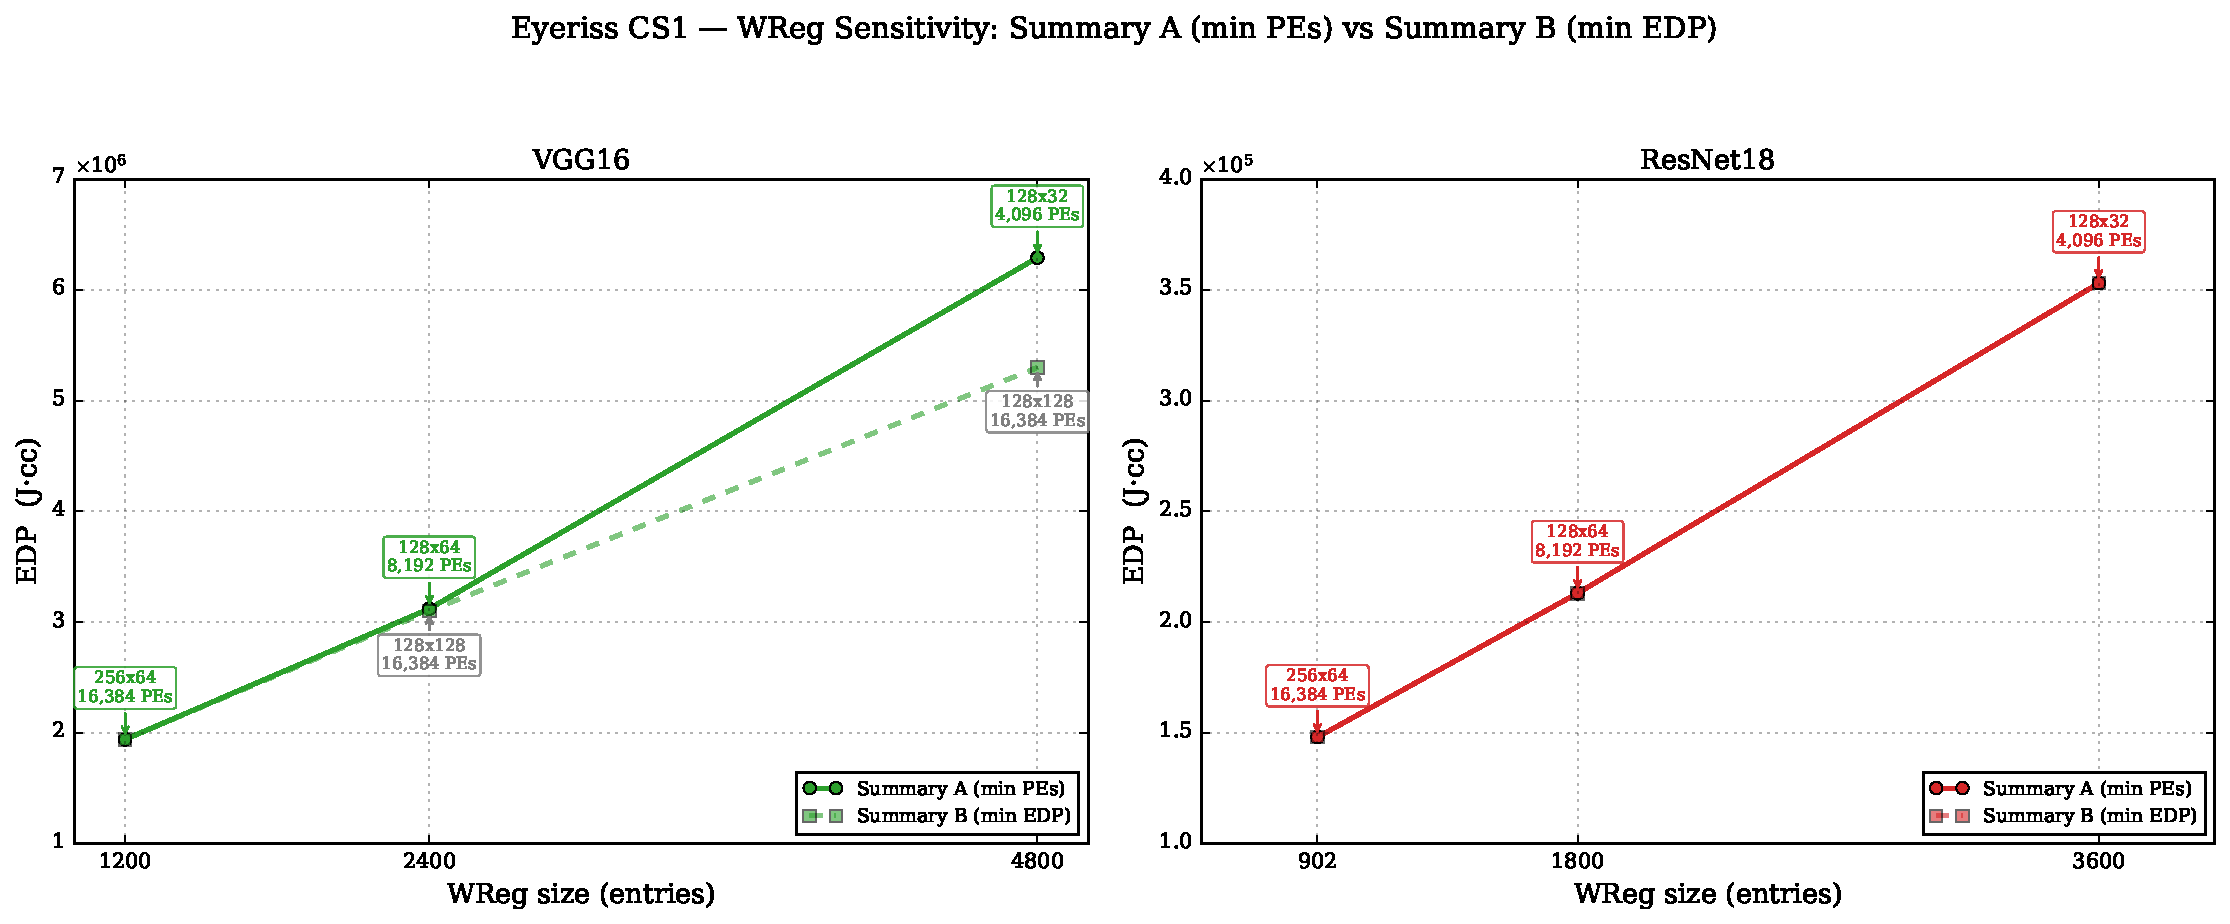
\includegraphics[width=0.85\textwidth]{plots/eyeriss_cs1_wreg_sweep.pdf}
  \caption{Eyeriss CS1 — EDP vs.\ WReg size for VGG16 and ResNet18.
    Summary~A selects the configuration with the fewest PEs; Summary~B
    selects the one with the lowest EDP.}
  \label{fig:ey-cs1-sweep}
\end{figure}

In both workloads, energy increases monotonically with WReg size
because a larger register incurs more read and write energy per
access.
For ResNet18, Summary~A and Summary~B coincide at all three WReg
sizes, meaning the minimum-PE configuration is also the minimum-EDP
one.
For VGG16, the two summaries diverge at WReg\,$\geq$\,2\,400: at
WReg\,=\,2\,400, Summary~A selects $128 \times 64$ (8\,192~PEs,
EDP\,=\,$3.12 \times 10^{6}$), while Summary~B selects
$128 \times 128$ (16\,384~PEs, EDP\,=\,$3.10 \times 10^{6}$), a
marginal improvement obtained at the cost of twice as many PEs.
This confirms that, once the WReg is large enough, the EDP benefit of
additional PEs is negligible.

For FSRCNN and MC-CNN, the WReg sweep is non-binding: all tested sizes
yield the same PE configuration and identical latency, so EDP scales
linearly with the register energy overhead.

\paragraph{Key takeaway.}
The WReg size is the primary feasibility constraint in the
Eyeriss-Like architecture under layer fusion.
Its sizing involves a three-way trade-off: a larger WReg reduces the
minimum PE count (saving area) but increases per-access register
energy, while a smaller WReg demands more PEs but keeps register
energy low.
For weight-dominant workloads such as VGG16 and ResNet18, the
constraint is tight: the smallest feasible WReg already requires the
maximum tested PE count (16\,384), and only two configurations are
viable.
For activation-dominant workloads the constraint is looser, and the
WReg choice affects only energy, not feasibility.
